\chapter{The observation of $^8$\ce{B} solar neutrino}
\label{chap:solar}

\section{Signal screening}
\label{sec:signal_screening}
\subsection{The dataset}
In order to search for $^8$\ce{B} solar neutrinos, we used the data from the MM trigger. During the data acquisition process in the water phase, the detector and the trigger system were still in the commissioning phase. Consequently, the data acquisition conditions were unstable. As a result, only a limited amount of data was available for the search of $^8$\ce{B} solar neutrinos. To address this, we carefully selected datasets with relatively high data acquisition quality and, to the greatest extent possible, performed calibrations both before and after data acquisition. Afetr selection, there were 9 runs in total, and the information of each run is shown in the Tab.~\ref{tab:summaryOfRuns_solar}. The total lifetime is \SI{18.13}{h} and more than \SI{15}{h} of data were taken at night.
\begin{table}[htbp]
	\centering
	\caption{The runs used for $^8$\ce{B} solar neutrinos}%标题
	\label{tab:summaryOfRuns_solar}
	\begin{tabular}{cccc}
		\toprule
		Run number & lifetime~($\text{h}$) & Time~(date/h) & MM Trigger threshold \\
		\midrule
		3322       & 1.15                  & 0203/00       & threshold=53         \\
		3323       & 0.69                  & 0203/01       & threshold=53         \\
		3413       & 2.76                  & 0203/23       & threshold=53         \\
		3415       & 0.48                  & 0204/03       & threshold=54.5       \\
		3416       & 3.20                  & 0204/03       & threshold=54.5       \\
		3530       & 1.43                  & 0205/23       & threshold=46.5       \\
		3531       & 1.34                  & 0206/01       & threshold=46.5       \\
		3639       & 2.18                  & 0207/17       & threshold=47         \\
		3677       & 4.88                  & 0208/01       & threshold=44         \\
		\bottomrule
	\end{tabular}
\end{table}

\subsection{The selection in preliminary reconstruction}
Given that likelihood-based reconstruction is time-consuming, we conduct event selection based on preliminary reconstruction. This approach aims to eliminate certain dark noise background events and radioactive background events from the PMT surface. The criteria are in following.
\begin{itemize}
	\item Fiducial volume $r < \SI{17}{m}$
	\item isglass $< 0.5$
	\item score $>0.001$
	\item $p_z/p>-0.8$
	\item $n_{20}>12$
\end{itemize}

\subsection{The energy selection}
In the water phase, $^8$\ce{B} solar neutrinos engage in elastic scattering~(ES) with electrons. As a result of this scattering process, the scattered electrons acquire energy and emit Cherenkov light, which is subsequently detected. Based on previous research, the mass of electron neutrinos is found to be less than \SI{0.31}{eV} at \SI{90}{\%} CL~\cite{KATRIN}. When observing neutrinos within the \si{MeV} energy range, the kinetic energy \(E_{k,\nu}\) is significantly greater than mass \(E_{\nu}\), i.e., \(E_{k,\nu} >> E_{\nu}\). During the calculation in ES, the mass of the neutrino itself can be neglected. Under such circumstances, the neutrino can be equivalently treated as Gamma. Consequently, the screening conditions can be derived from the calibration of the Gamma source, enabling us to determine the reasonableness of the remaining events.
From Sec.~\ref{subsec:low_energy}, we can get the relationship between Gamma energy and $n_{20}$ is $n_{20}=14E+8.1$. When the energy scale of Gamma is applied to neutrinos, it becomes possible to directly bypass the recoil electrons, directly estimate the corresponding neutrino energy and optimize the selection of neutrino signals.
As shown in Fig.~\ref{fig:solar_n20_select}, we have a cut of energy: $93<n_{20}<233$, corresponding to the neutrino energy range of 6.1 -- \SI{16}{MeV}.
\begin{figure}[htbp]
	\centering
	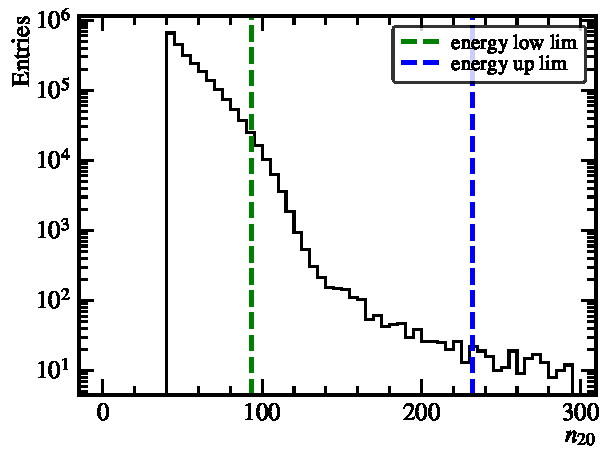
\includegraphics[width=0.5\textwidth]{solarSearch/n20Cut.pdf}
	\caption{The selection of energy of $^8$\ce{B} solar neutrinos.}
	\label{fig:solar_n20_select}
\end{figure}

\subsection{The position selection}
Following the energy screening, it was observed that a substantial number of events converged at the center of the detector, as shown in Fig.~\ref{fig:solar_pos_cut}. Analogous to the scenario depicted in Fig.~\ref{fig:solar_direction}, the events at the center exhibited a downward tendency. Given that the search for $^8$\ce{B} solar neutrinos is highly direction-dependent, rather than implementing a direction cut, we chose an additional cylindrical region at the center of the detector for screening, as illustrated in Fig.~\ref{fig:solar_pos_cut}. Our final FV cut is:
\begin{itemize}
	\item $x^2+y^2>50$~\si{m^2}
	\item $r<14$~\si{m}
\end{itemize}

\begin{figure}[htbp]
	\centering
	\begin{subfigure}{0.5\textwidth}
		\centering
		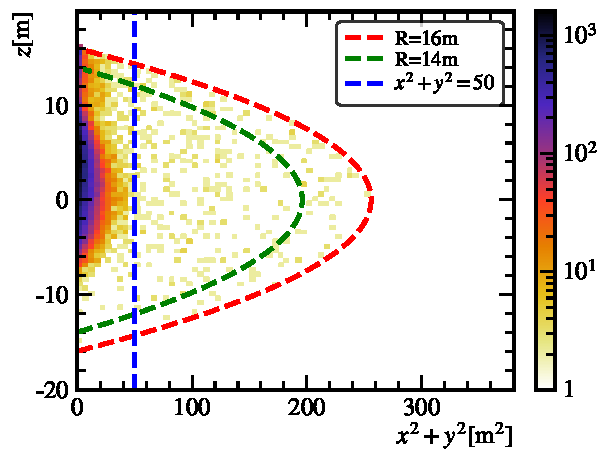
\includegraphics[width=0.9\textwidth]{solarSearch/Position_Cut.pdf}
		\caption{}
		\label{fig:solar_pos_cut}
		% 图片宽度占子图宽度的80%
	\end{subfigure}% 
	\begin{subfigure}{0.5\textwidth}
		\centering
		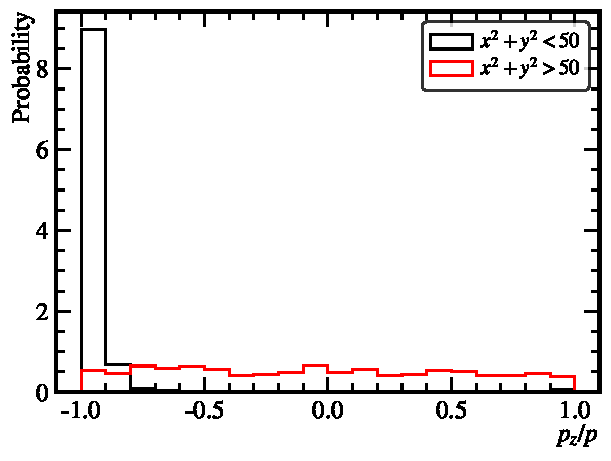
\includegraphics[width=0.9\textwidth]{solarSearch/pzp_FV.pdf}
		\caption{}
		\label{fig:solar_direction}
	\end{subfigure}
	\caption{The position selection of $^8$\ce{B} solar neutrino. \subref{fig:solar_pos_cut} shows the final FV selection, while \subref{fig:solar_direction} shows direction distribution in different regions.}
	\label{fig:solar_position_cut}
\end{figure}

\subsection{The muon spallation cut}
For $^8$\ce{B} solar neutrinos, the most significant background comes from the electrons produced by the decay of radioactive isotopes generated by the reaction of cosmic muons with oxygen atoms. JUNOsw was employed to simulate 500,000 muons going through the CD. A statistical analysis was conducted on the generated neutrons and spallation isotops, along with the electrons and Gammas from their decay. Based on the neutron yield measured in the water phase, the approximate yields of various isotopes in water were calculated, as shown in Tab.~\ref{tab:solar_spallation_bkg}. The distance between them and muons are illustrated Fig.~\ref{fig:solar_isotops}.
For isotopes with a lifetime less than \SI{300}{ms}, we can remove them by analyzing the relative positions of muons within \SI{1}{s}. However, for isotopes with a lifetime longer than \SI{1}{s}, it is difficult to remove them through simple methods. The sum of the yields of long-lifetime spallation isotops is $21.159\times 10^{-7}~\mu^{-1}\mathrm{g}^{-1}\mathrm{cm}^{2}$. The electrons and Gammas with energies ranging from 5 to \SI{20}{MeV} generated by their decay will seriously influence the search for $^8$\ce{B} solar neutrino signals, and this part of events accounts for \SI{29.5}{\%} of the total number of generated events. After the reconstruction, the total length of the muon track is $l_{\mu}=5.8\times10^8~\text{cm}$ and the expectation of those events is 362. Considering that the neutron yield has an uncertainty of \SI{20}{\%}, and after neglecting the uncertainty of muon reconstruction, the expected background count is $362\pm69$ without any cut.

\begin{table}[htbp]
	\centering
	\caption{The main types of spallation isotopes and the primary processes that produce them~\cite{spallation_isotops}. We use the measured yield of spallation neutrons to scale the yields of other isotopes based on simulation.}%标题
	\label{tab:solar_spallation_bkg}
	\begin{tabular}{ccccccc}
		\toprule
		Isotope       & Lifetime & Decay mode        & Energy               & $N_{sim}$ & Scaled Yield                                      \\
		              & (\si{s}) &                   & (\si{MeV})           &           & ($10^{-7}\mu^{-1}\mathrm{g}^{-1}\mathrm{cm}^{2}$) \\
		\midrule
		n             & 0.0002   & n-H               & 2.2                  & 266910    & 2310                                              \\
		\addlinespace
		$^{11}_{4}$Be & 19.9     & $\beta^{-}$       & 11.51                & 47        & 0.407                                             \\
		              &          & $\beta^{-}\gamma$ & 9.41+2.1($\gamma$)   &           &                                                   \\
		\addlinespace
		$^{16}_{7}$N  & 10.3     & $\beta^{-}$       & 10.44                & 2003      & 17.334                                            \\
		              &          & $\beta^{-}\gamma$ & 4.27+6.13($\gamma$)                                                                  \\
		\addlinespace
		$^{15}_{6}$C  & 3.53     & $\beta^{-}$       & 9.77                 & 294       & 2.544                                             \\
		              &          & $\beta^{-}\gamma$ & 4.51+5.30($\gamma$)                                                                  \\
		\addlinespace
		$^{8}_{3}$Li  & 1.21     & $\beta^{-}$       & $\sim$13.0           & 78        & 0.675                                             \\
		\addlinespace
		$^{8}_{5}$B   & 1.11     & $\beta^{+}$       & $\sim$13.9           & 23        & 0.199                                             \\
		\addlinespace
		$^{9}_{3}$Li  & 0.26     & $\beta^{-}$       & 13.6                 & 42        & 0.363                                             \\
		              &          & $\beta^{-}$+n     & $\sim$10                                                                             \\
		\addlinespace
		$^{9}_{6}$C   & 0.18     & $\beta^{+}$+p     & 3-15                 & 6         & 0.052                                             \\
		\addlinespace
		$^{8}_{2}$He  & 0.17     & $\beta^{-}\gamma$ & 9.67+0.98($\gamma$)  & 4         & 0.034                                             \\
		              &          & $\beta^{-}$+n     &                                                                                      \\
		\addlinespace
		$^{12}_{4}$Be & 0.034    & $\beta^{-}$       & 11.71                & 72        & 0.623                                             \\
		\addlinespace
		$^{12}_{5}$B  & 0.029    & $\beta^{-}$       & 13.37                & 800       & 6.923                                             \\
		\addlinespace
		$^{13}_{5}$B  & 0.025    & $\beta^{-}$       & 13.44                & 457       & 3.955                                             \\
		\addlinespace
		$^{14}_{5}$B  & 0.02     & $\beta^{-}\gamma$ & 14.55+6.09($\gamma$) & 277       & 2.397                                             \\
		\addlinespace
		$^{12}_{7}$N  & 0.016    & $\beta^{+}$       & 16.38                & 250       & 2.164                                             \\
		\addlinespace
		$^{13}_{8}$O  & 0.013    & $\beta^{+}$+p     & 8-14                 & 167       & 1.445                                             \\
		\addlinespace
		$^{11}_{3}$Li & 0.012    & $\beta^{-}$       & 20.62                & 2         & 0.017                                             \\
		              &          & $\beta^{-}$+n     & $\sim$16                                                                             \\
		\bottomrule
	\end{tabular}
\end{table}

\begin{figure}[htbp]
	\centering
	\begin{subfigure}{0.5\textwidth}
		\centering
		\includegraphics[page=10, width=0.9\textwidth]{solarSearch/iso.pdf}
		\caption{}
		\label{fig:solar_isotops}
	\end{subfigure}%
	\begin{subfigure}{0.5\textwidth}
		\centering
		\includegraphics[page=11, width=0.9\textwidth]{solarSearch/iso.pdf}
		\caption{}
		\label{fig:solar_gamma_electron}
	\end{subfigure}
	\caption{The distribution of the distance between spallation isotopes~\subref{fig:solar_isotops},  electrons  or Gammas~\subref{fig:solar_gamma_electron} and the muon track.}
	\label{fig:solar_isotops_all}
\end{figure}
Taking into account the resolution of the reconstruction, position cuts were implemented on the spallation background, which was then partitioned into two components:
\begin{itemize}
	\item Time cut: >\SI{5}{ms} after muon
	\item Position cut: >\SI{15}{m} from muon track if there is a muon before events in 1--\SI{1000}{ms}, as shown in Fig.~\ref{fig:solar_spallation_cut}.
\end{itemize}

\begin{figure}[htbp]
	\centering
	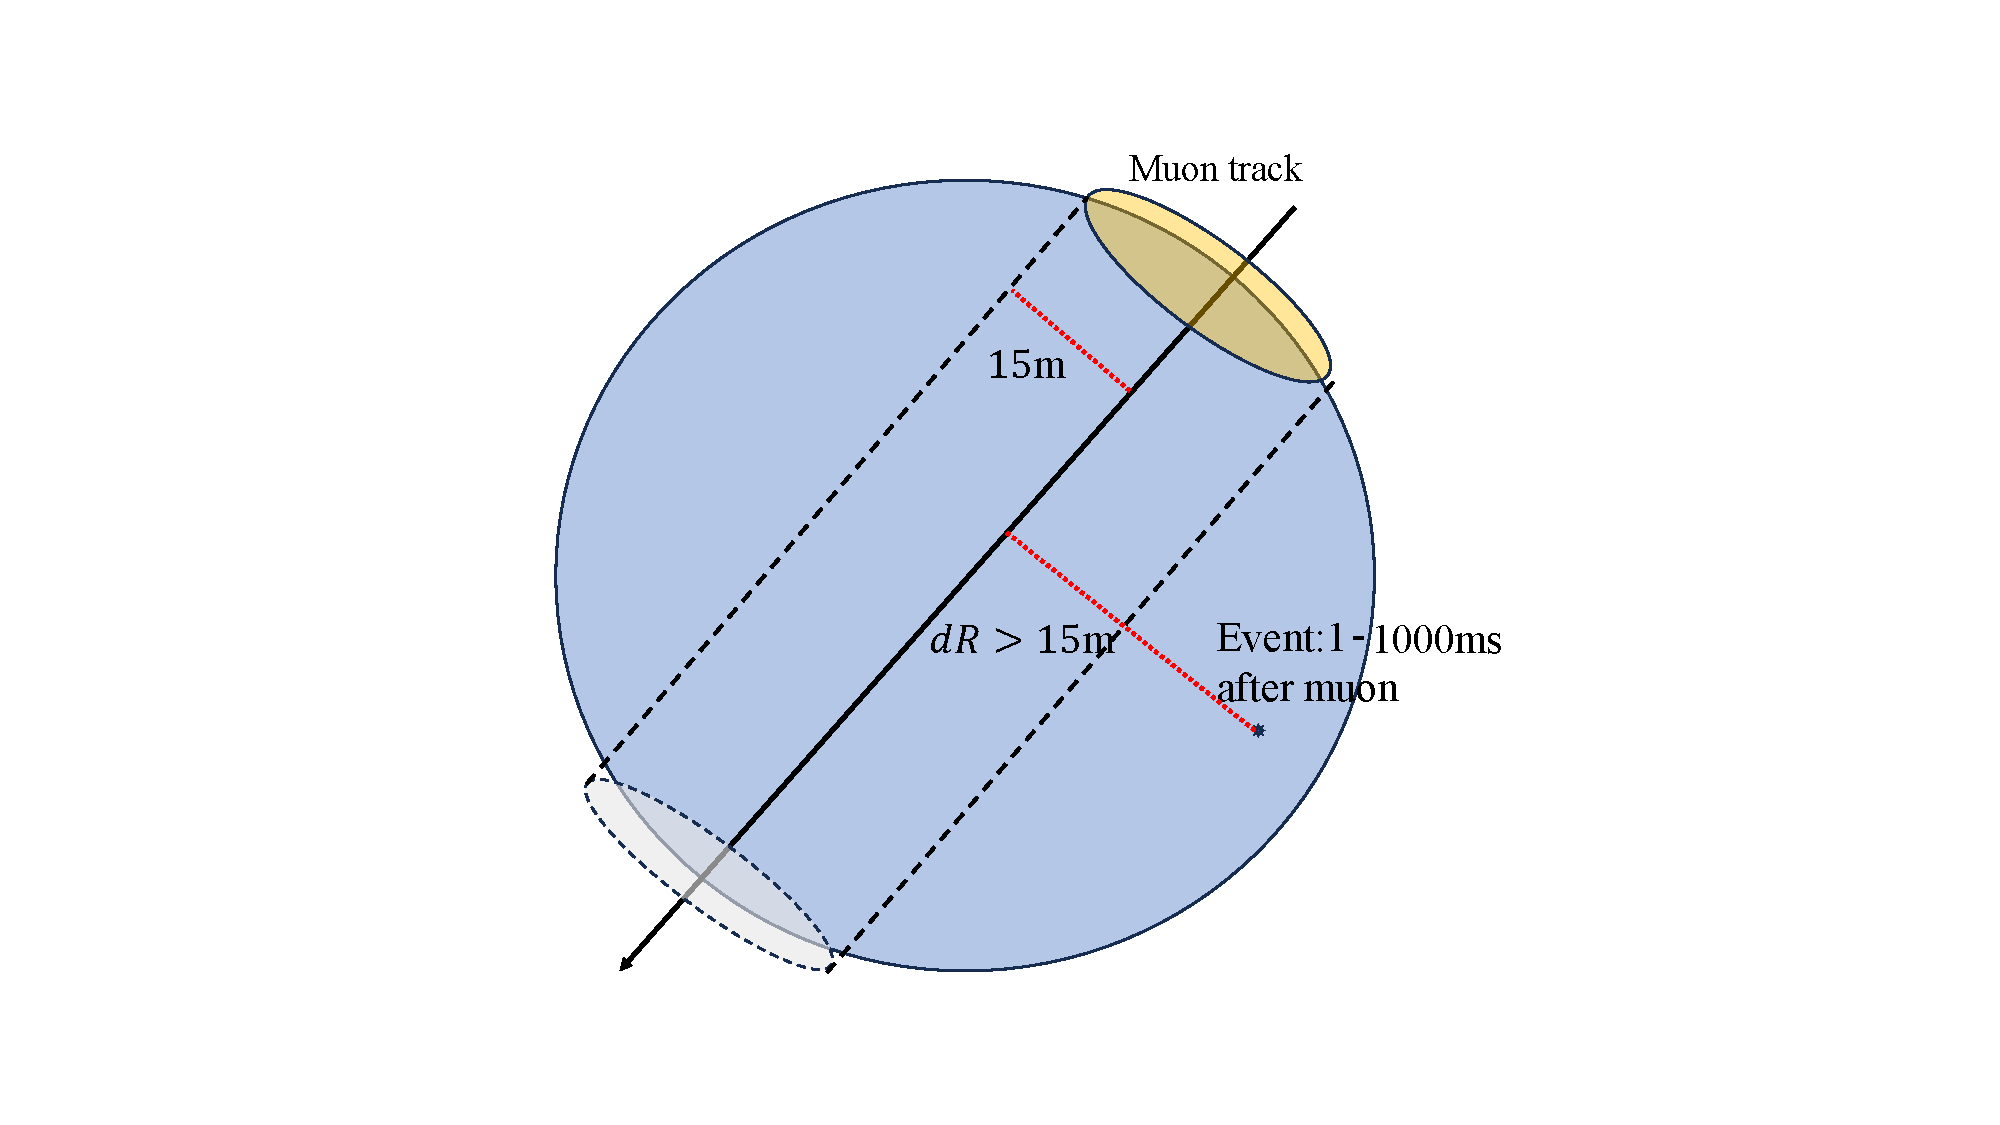
\includegraphics[width=0.5\textwidth]{solarSearch/spallation_cut.pdf}
	\caption{The position cut of spallation background.}
	\label{fig:solar_spallation_cut}
\end{figure}

\subsection{The summary of selections}
In addition to those cuts before, we have cut on goodness $G_{vd}$ and Cherenkov ring quality $n_c/n_{20}$. All the cut we used for $^8$\ce{B} solar neutrinos are in Tab.~\ref{tab:selection_summary}.
\begin{table}[htbp]
	\centering
	\caption{The final selection for $^8$\ce{B} solar neutrinos}%标题
	\label{tab:selection_summary}
	\begin{tabular}{ccc}
		\toprule
		                & selection conditions                                  \\
		\midrule
		Fiducial volume & r<\SI{14}{m}                                          \\
		                & $x^2+y^2>50~\text{m}^2$                               \\
		Energy          & $93<n_{20}<233$                                       \\
		Quality         & $n_c/n_{20}>0.23$                                     \\
		                & $G_{vd}>0.29$                                         \\
		Spallation cut  & >\SI{5}{ms} after muon                                \\
		                & >\SI{15}{m}, if muon in 1--\SI{1000}{ms} before event \\
		\bottomrule
	\end{tabular}
\end{table}

\section{The observation of $^8$\ce{B} solar neutrino signals}
\subsection{Definition of the solar angle}
Solar neutrinos are produced in the core of the Sun. During the process of ES, the directional properties of neutrinos are maintained. Therefore, the number of $^8$\ce{B} solar neutrino events can be estimated by calculating the angle between the direction of the events and the azimuth of the Sun, that is, the solar angle~($\theta_s$), as shown in Fig.~\ref{fig:solar_angle_define}.
\begin{figure}[htbp]
	\centering
	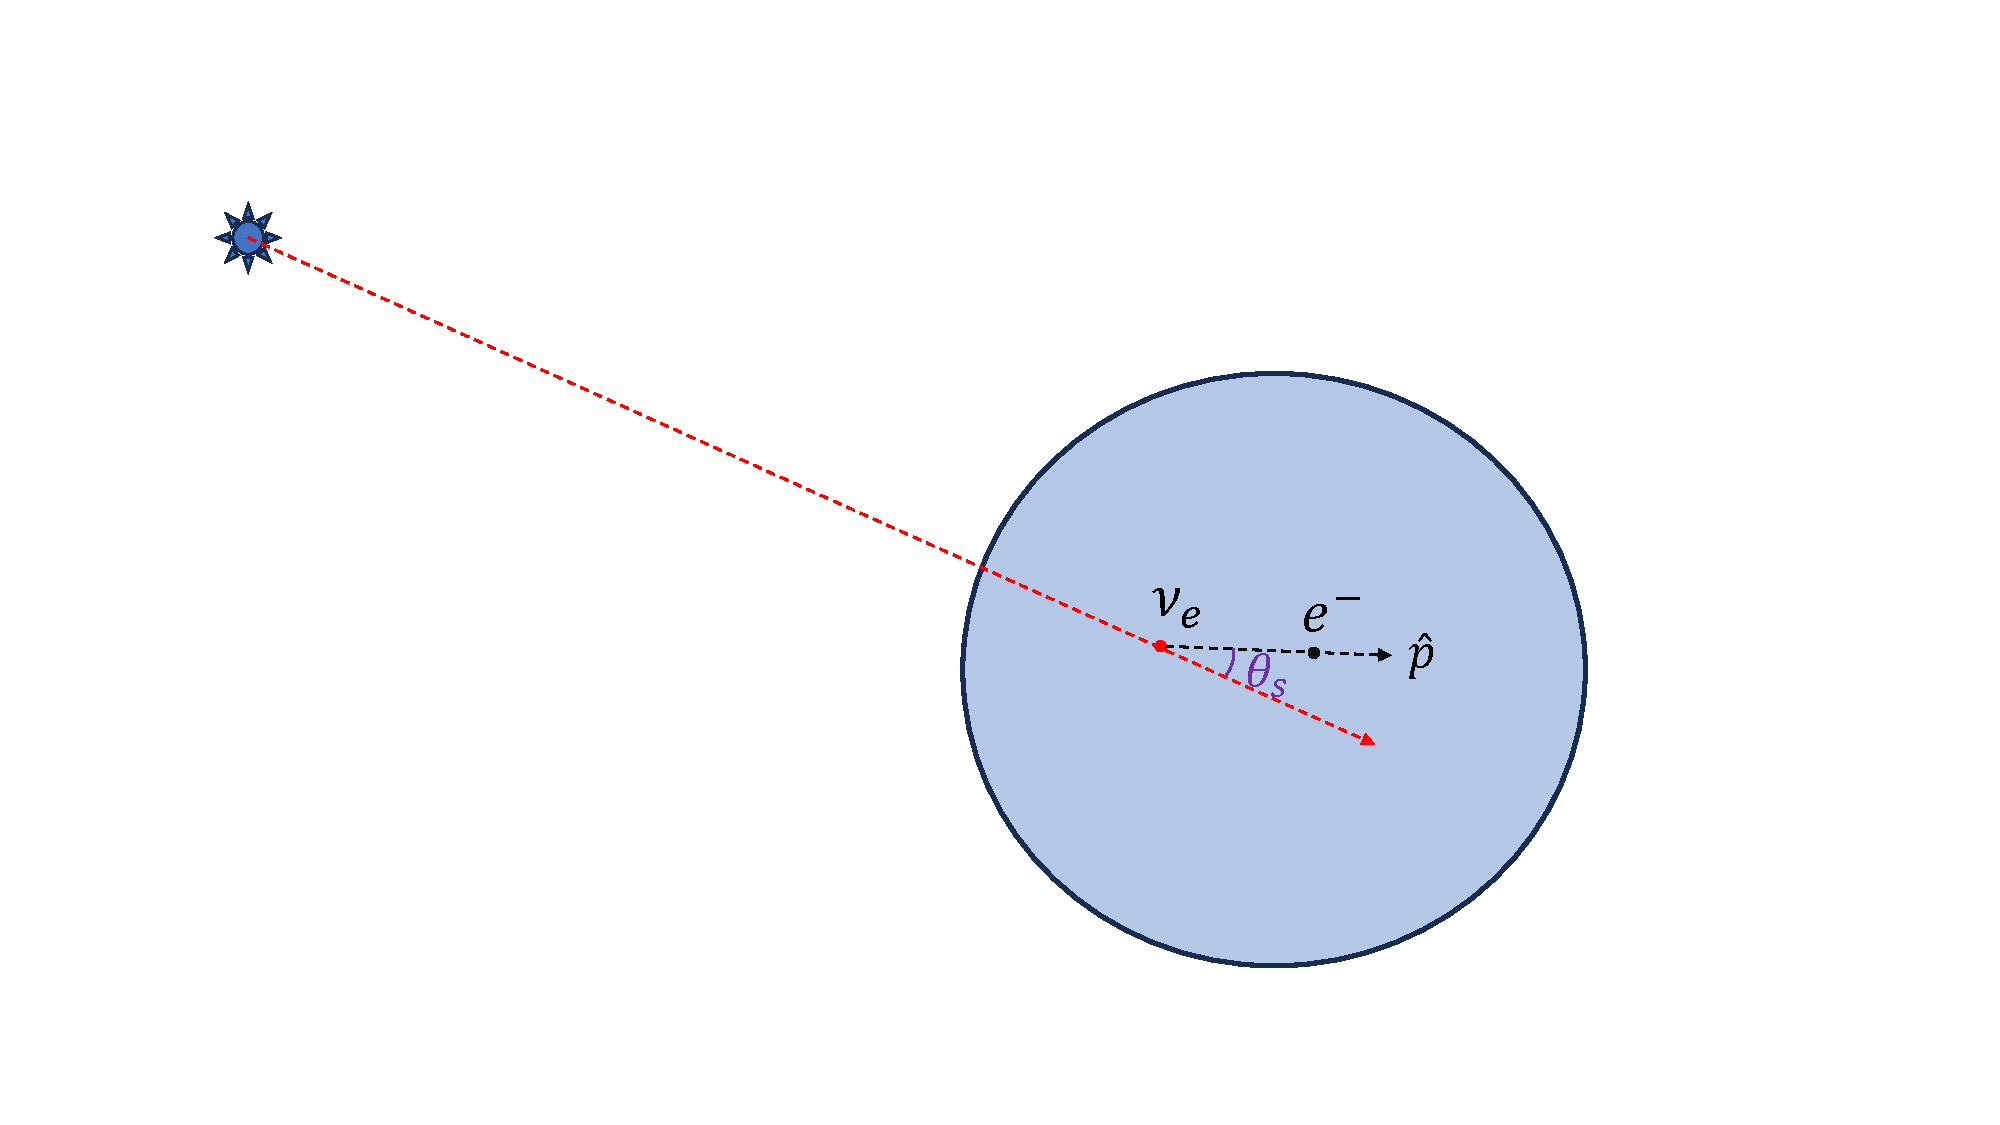
\includegraphics[width=0.7\textwidth]{solarSearch/solarAngleDef.pdf}
	\caption{The definition of solar angle.}
	\label{fig:solar_angle_define}
\end{figure}
\subsection{The observation of $^8$\ce{B} solar neutrinos}
\label{sec:solar_observation}
After the selections in Sec.~\ref{sec:signal_screening}, we can get the solar angle distribution as shown in Fig.~\ref{fig:solar_angle}, and their position distribution as illustrated in Fig.~\ref{fig:solar_pos}.
\begin{figure}[htbp]
	\centering
	\begin{subfigure}{0.5\textwidth}
		\centering
		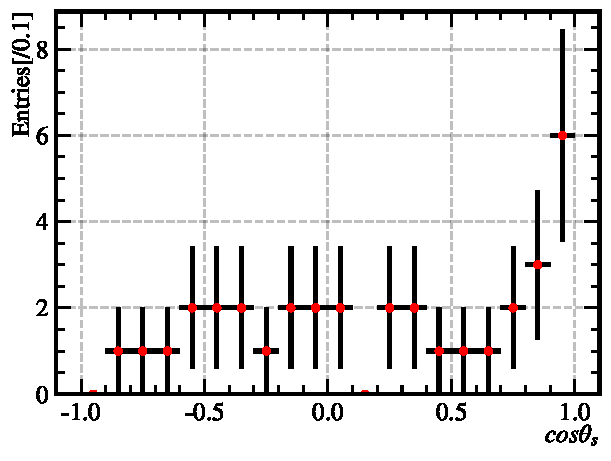
\includegraphics[width=0.9\textwidth]{solarSearch/SolarAngle_err.pdf}
		\caption{}
		\label{fig:solar_angle}
	\end{subfigure}%
	\begin{subfigure}{0.5\textwidth}
		\centering
		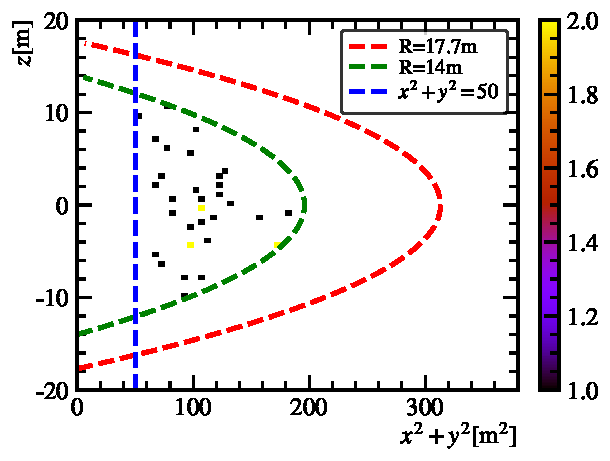
\includegraphics[width=0.9\textwidth]{solarSearch/Position_Cut_final.pdf}
		\caption{}
		\label{fig:solar_pos}
	\end{subfigure}
	\caption{The distribution of solar angle~\subref{fig:solar_angle},  and position distribution of $^8$\ce{B} solar neutrino candidates~\subref{fig:solar_pos}.}
	\label{fig:solar_final_distribution}
\end{figure}

To check whether the distribution of the solar angle is reasonable, we still use Gamma for approximation. In the Compton scattering of Gamma and electrons, the electrons also possess the directional characteristics of Gamma. We can define the Gamma angle in a way similar to the solar angle, as illustrated in Fig.~\ref{fig:solar_gamma_angle}. We applied the same energy cut and quality cut to the calibration source as those employed in the search for $^8$\ce{B} solar neutrinos. A clear peak can be seen at $\cos\theta_{\gamma}=1$, as shown in Fig.~\ref{fig:solar_gamma_dis}, which indicates that we have indeed detected the $^8$\ce{B} solar neutrino signal in water phase.

\begin{figure}[htbp]
	\centering
	\begin{subfigure}{0.5\textwidth}
		\centering
		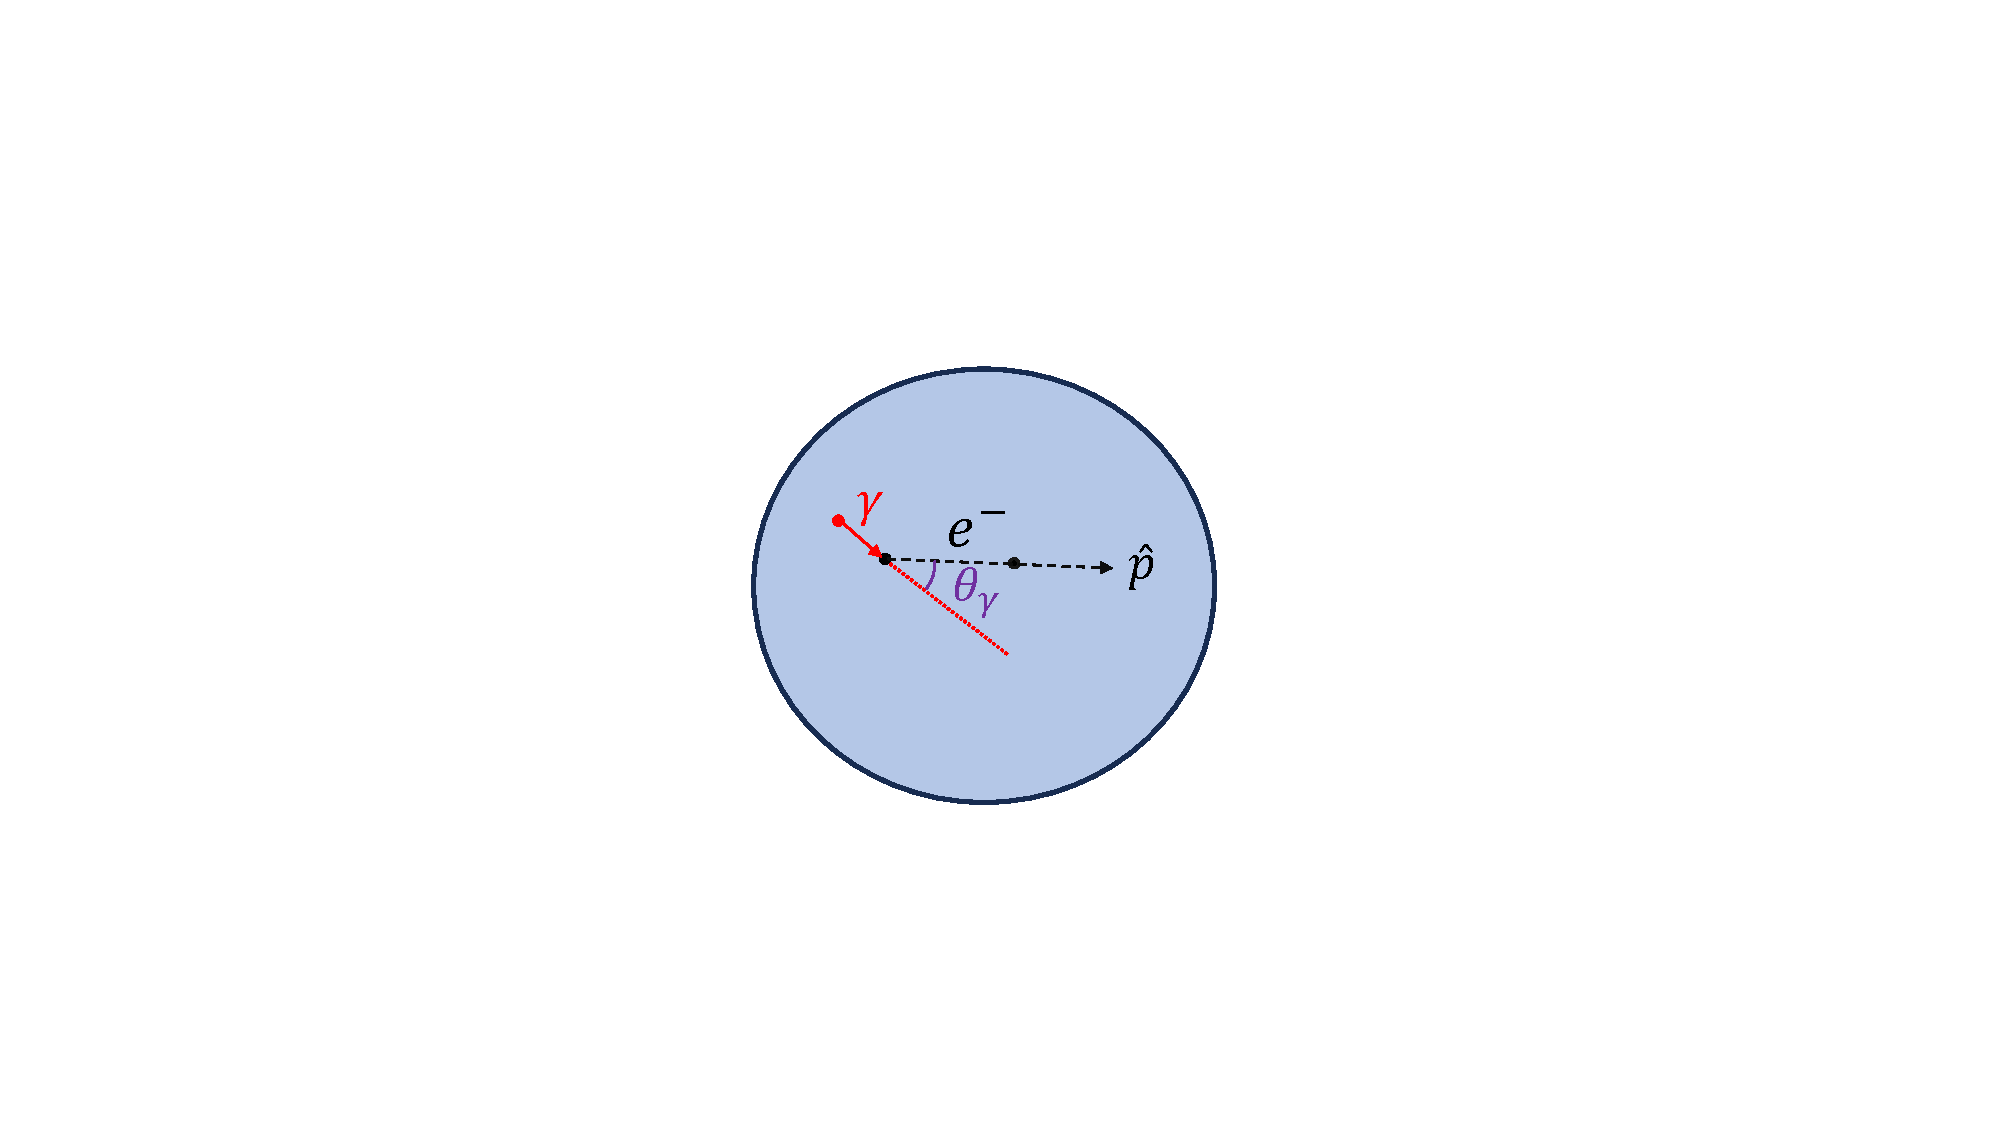
\includegraphics[height=4.5cm]{solarSearch/gamma_angle.pdf}
		\caption{}
		\label{fig:solar_gamma_angle}
	\end{subfigure}%
	\begin{subfigure}{0.5\textwidth}
		\centering
		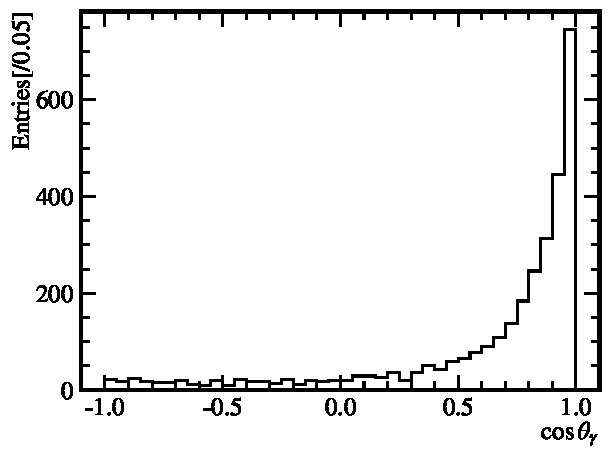
\includegraphics[height=4.5cm]{solarSearch/gamma_angle_3286.pdf}
		\caption{}
		\label{fig:solar_gamma_dis}
	\end{subfigure}
	\caption{\subref{fig:solar_gamma_angle}:The definition of Gamma angle~\subref{fig:solar_gamma_angle}. \subref{fig:solar_gamma_dis}: The distribution of $\cos\theta_{\gamma}$ in calibration Run~3286.}
	\label{fig:solar_final_gamma_angle}
\end{figure}

We can use the bins with $\cos\theta_s > 0.5$ as the signal interval and obtain 13 candidates for the signal. The bins with $\cos\theta_s < 0$ are used to estimate the background level, which is 1.3 in each bin. Finally, the number of $^8$\ce{B} solar neutrino signals obtained is $N_s=6.50\pm2.54$, along with $26.0\pm5.1$ backgrounds.

\section{The estimation of $^8$\ce{B} solar neutrino flux}
\label{sec:solar_flux}
We can use Eq.~\eqref{eq:flux} to estimate the flux of $^8$\ce{B} neutrino.
\begin{equation}
	\phi_{B8}=\frac{N_s}{N_e\sigma_t t_f \eta_s}
	\label{eq:flux}
\end{equation}
Where $N_s$ is the number of solar $^8$\ce{B} neutrino, $\sigma_t$ is the total cross section of ES, $N_e$ is the number of electrons, $t_f$ is the exposure time and $\eta_s$ is the efficiency, including the FV and other selections.

\subsection{The flux estimation}
The total number of electrons can be obtained through mathematical calculations:
\begin{equation}
	N_e=\frac{4\pi}{3}\times (1770~\text{cm})^3\times 1~\text{g}/\text{cm}^3\times \frac{1}{18}~\text{mol}/\text{g}\times N_A\times 10=7.77\times10^{33}
\end{equation}

Combining the $^8$\ce{B} neutrino energy distribution mearsured by Winter et al.~\cite{B8_winter} as evidenced in Fig.~\ref{fig:solar_B8_err_e} and the cross section calculated by Bachall~\cite{Bahcall_correct} as shown in Fig.~\ref{fig:solar_B8_cross}, we get the total cross section: $\sigma_t=5.82\times10^{-44}~\text{cm}^2$.
\begin{figure}[htbp]
	\centering
	\begin{subfigure}{0.5\textwidth}
		\centering
		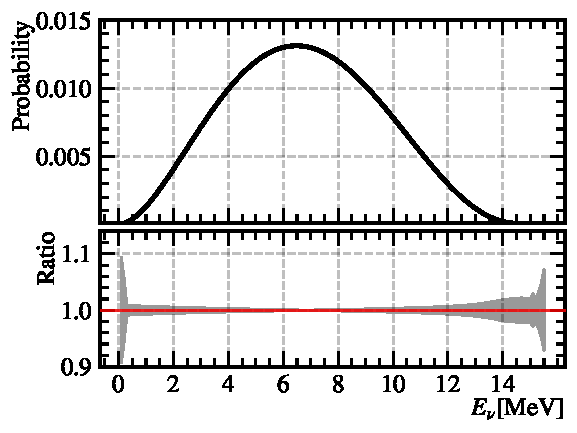
\includegraphics[width=0.9\textwidth]{solarSearch/B8_spectrum_err_e.pdf}
		\caption{}
		\label{fig:solar_B8_err_e}
	\end{subfigure}%
	\begin{subfigure}{0.5\textwidth}
		\centering
		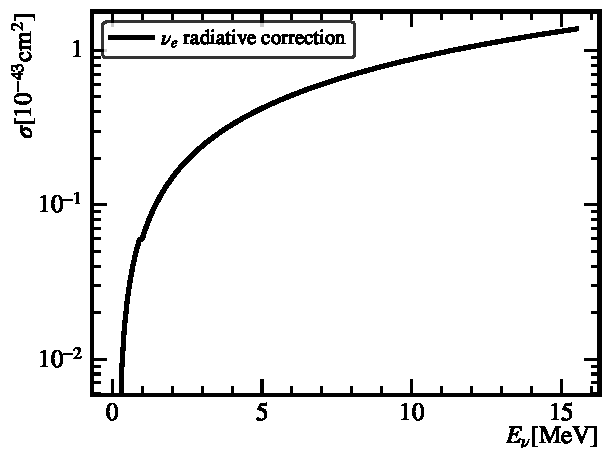
\includegraphics[width=0.9\textwidth]{solarSearch/B8_spectrum_cross.pdf}
		\caption{}
		\label{fig:solar_B8_cross}
	\end{subfigure}
	\caption{\subref{fig:solar_B8_err_e} shows the energy distribution and the systematic uncertainty of spectrum shape of $^8$\ce{B} neutrino, and the data comes from~\cite{B8_winter}. \subref{fig:solar_B8_cross} shows the cross section of ES and the calculation comes from~\cite{Bahcall_correct}.}
\end{figure}

The efficiency $\eta$ can be calculated by combing simulation and source calibrations. We simulated 75000 $^8$\ce{B} solar neutrinos uniformly in CD and the energy distribution of neutrinos and recoil electrons are as shown in Fig.~\ref{fig:solar_sim_info}. After applying all the selections mentioned in Sec.~\ref{sec:signal_screening}, we obtained an efficiency of $\eta_s=(8.98\pm0.11)~\%$. After deducting the muon veto, the effective exposure time is $t_f=17.64~\text{h}$.

\begin{figure}[htbp]
	\centering
	\begin{subfigure}{0.5\textwidth}
		\centering
		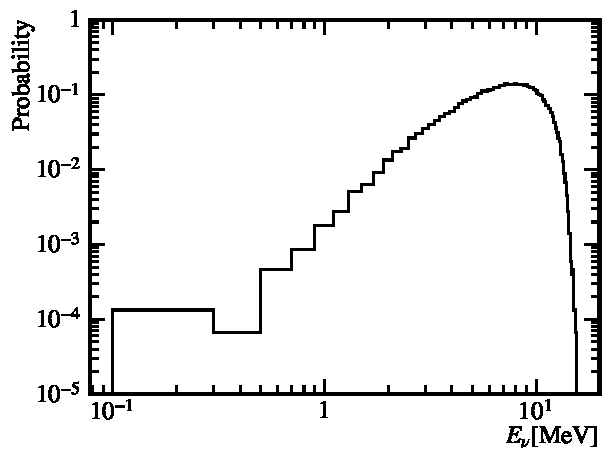
\includegraphics[width=0.9\textwidth]{solarSearch/E_nve.pdf}
		\caption{}
		\label{fig:solar_B8_sim_e}
	\end{subfigure}%
	\begin{subfigure}{0.5\textwidth}
		\centering
		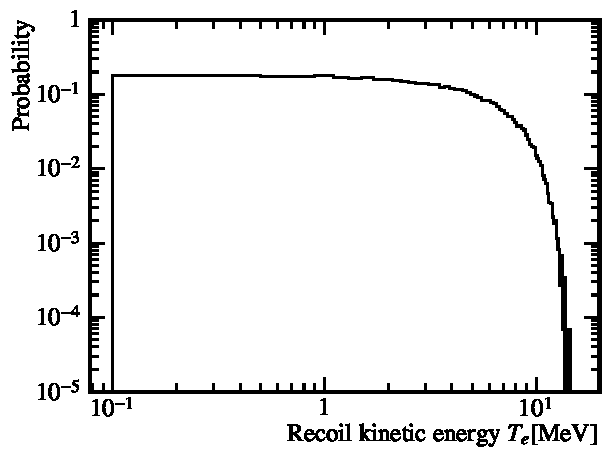
\includegraphics[width=0.9\textwidth]{solarSearch/Te.pdf}
		\caption{}
		\label{fig:solar_B8_sim_electron}
	\end{subfigure}
	\begin{subfigure}{0.5\textwidth}
		\centering
		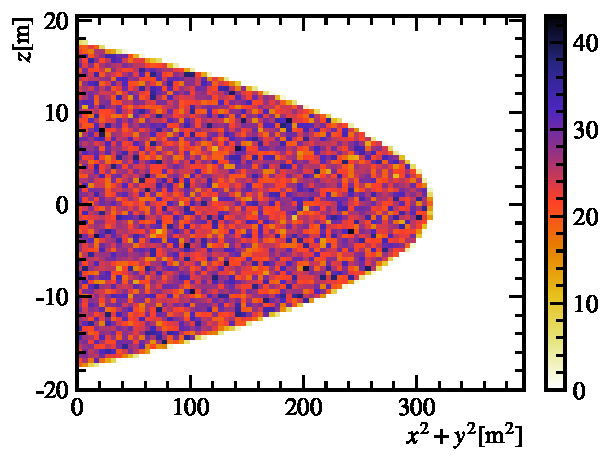
\includegraphics[width=0.9\textwidth]{solarSearch/Sim_e_Pos.pdf}
		\caption{}
		\label{fig:solar_B8_sim_electron_pos}
	\end{subfigure}
	\caption{\subref{fig:solar_B8_sim_e} depicts the energy distribution of captured $^8$\ce{B} neutrinos. \subref{fig:solar_B8_sim_electron} presents that of the recoil electrons, and \subref{fig:solar_B8_sim_electron} represents the position distribution.}
	\label{fig:solar_sim_info}
\end{figure}

Finally, we can estimate the flux of $^8$\ce{B} solar neutrino: $$\phi_{B8}=(2.52\pm0.99)\times10^6~\text{cm}^{-2}\text{s}^{-1}$$

\subsection{The systematic uncertainty}
Due to the lack of detailed graduations, our estimation of systematic errors is rather rough. We ignore the systematic uncertainties in exposure time and the number of electrons, and only consider the uncertainty of the energy spectrum as well as the differences between simulation and data. For the energy spectrum, we consider the uncertainty of the shape of the energy spectrum, as shown in Fig.~\ref{fig:solar_B8_err_e}. By adjusting the energy distribution within the error range and recalculating the total cross section, we find that the uncertainty caused by this factor is less than\SI{1}{\%}.
For the differences between simulation and data, we selected events in calibration Run 3281, 3283 and 3286 to compare with simulation.
We selected events within \SI{5}{m} around the calibration source. The requirements are that the direction should satisfy $p_z/p > - 0.6$ and $n_{10}-n_{b}>22$. After applying the same energy cut and quality cut as those used in the search for $^8$\ce{B} solar neutrinos, we obtained the remained events ratio as efficiency. We simulated 6.1 MeV gamma rays at the same position and calculated the corresponding efficiency. The results of both are shown in Fig.~\ref{fig:solar_efficiency}. The efficiency in data is \SI{34.9}{\%}, while that in simulation is \SI{37.5}{\%}. The difference between them is \SI{7.44}{\%}, which we take as the systematic uncertainty of efficiency. Finally, the total systematic uncertainty is \SI{7.52}{\%}. The final flux is:$$\phi_{B8}=(2.52\pm0.19(\text{sys.})\pm0.99(\text{stat.}))\times10^6~\text{cm}^{-2}\text{s}^{-1}$$
\begin{figure}[htbp]
	\centering
	\begin{subfigure}{0.5\textwidth}
		\centering
		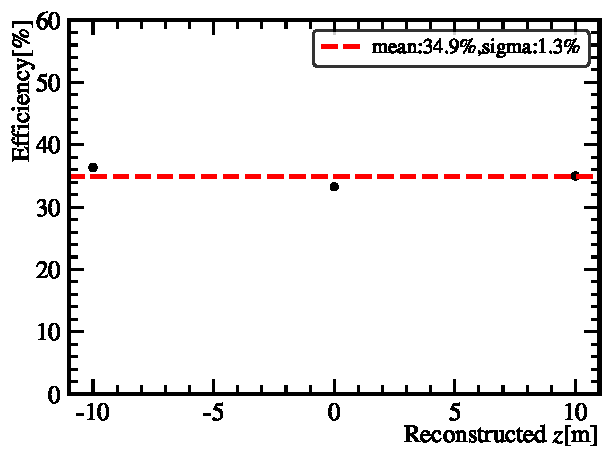
\includegraphics[width=0.9\textwidth]{solarSearch/eff_err_data.pdf}
		\caption{}
		\label{fig:solar_efficiency_data}
	\end{subfigure}%
	\begin{subfigure}{0.5\textwidth}
		\centering
		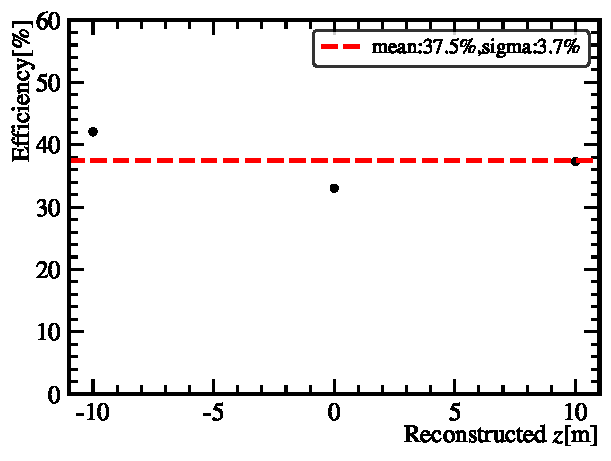
\includegraphics[width=0.9\textwidth]{solarSearch/eff_err_sim.pdf}
		\caption{}
		\label{fig:solar_efficiency_sim}
	\end{subfigure}
	\caption{\subref{fig:solar_efficiency_data} depicts the estimated efficiency in source calibration. \subref{fig:solar_efficiency_sim} presents that in simulation.}
	\label{fig:solar_efficiency}
\end{figure}
Meanwhile, we apply the estimated efficiency of the cut from the calibrations and calculate the ratio of FV to estimate the final number of backgrounds:
\begin{equation}
	N_b=362\times(1\pm0.2)\times\frac{14^3-50\times14\times2}{17.7^3}\times34.9\%=30.62\pm6.12
	\label{eq:solar_background_final}
\end{equation}
The result is consistent with the background estimated from the solar angle distribution in Sec.~\ref{sec:solar_observation}.

\subsection{The survival probability of $^8$\ce{B} solar neutrinos}
The total flux of $^8$\ce{B} solar neutrinos measured by SNO~\cite{SNO5.25} is
$$\phi_{B8,tot}=5.25\times10^6~\text{cm}^{-2}\text{s}^{-1}$$
The survival probability of $^8$\ce{B} solar neutrinos can be calculated as
$$P_{ee}=\phi_{B8}/\phi_{B8,tot}=0.48\pm0.04(\text{sys.})\pm0.19(\text{stat.})$$
which verifies the existence of solar neutrino oscillations in the JUNO water phase.